\subsection{Model: Decision Tree}

\subsubsection{Introduction}
This report evaluates the performance of the Decision Tree model trained using various embedding methods. The model was implemented using the \texttt{DecisionTreeClassifier} class from scikit-learn, with different configurations such as maximum depth, minimum samples per split, and other hyperparameters. The primary goal was to achieve high classification accuracy while ensuring robust generalization across different embedding techniques.

\subsubsection{Training Configuration}

The Decision Tree model was trained with the following hyperparameter search space:

\begin{itemize}
    \item \textbf{criterion}:  ["gini", "entropy"],
    \item \textbf{max\_depth}: [10, 20, 30, 40],
    \item \textbf{min\_samples\_split}: [2, 5, 10],
    \item \textbf{min\_samples\_leaf}: [1, 2, 4],
    \item \textbf{max\_features}: ["sqrt", "log2"]
\end{itemize}

% The best hyperparameters selected based on model evaluation were:
% \begin{itemize}
%     \item \textbf{criterion}:  ["gini"],
%     \item \textbf{max\_depth}: [40],
%     \item \textbf{min\_samples\_split}: [10],
%     \item \textbf{min\_samples\_leaf}: [2],
%     \item \textbf{max\_features}: ["sqrt"]
% \end{itemize}

A grid or random search was performed over these hyperparameters, employing K-Fold Cross-Validation to select the best configuration. The final chosen hyperparameters were validated on a withheld test set.

\subsubsection{Training and Evaluation Results}

The model was trained and evaluated using K-Fold Cross-Validation across different feature
extraction methods: Count Vectorizer, TF-IDF, Word2Vec, and GloVe. The best model was
selected based on Accuracy, with secondary considerations for F1-score and ROC AUC.

\textbf{Training Performance Metrics:}

\begin{table}[H]
    \centering
    \caption{Training Performance Metrics for Decision Tree}
    \label{tab:lr-training-metrics}
    \begin{tabular}{|l|c|c|c|c|c|}
        \hline
        \textbf{Method} & \textbf{Accuracy} & \textbf{ROC AUC} & \textbf{F1} & \textbf{Precision} & \textbf{Recall} \\ 
        \hline
        Count Vectorizer & 0.60 & 0.59 & 0.69 & 0.57 & 0.85 \\ 
        \hline
        TF-IDF & 0.59 & 0.58 & 0.69 & 0.56 & 0.89 \\ 
        \hline
        Word2Vec & 0.61 & 0.61 & 0.61 & 0.62 & 0.60 \\ 
        \hline
        GloVe & 0.60 & 0.60 & 0.61 & 0.61 & 0.60 \\ 
        \hline
    \end{tabular}
\end{table}

\textbf{Testing Performance Metrics:}

\begin{table}[H]
    \centering
    \caption{Testing Performance Metrics for Decision Tree}
    \label{tab:lr-testing-metrics}
    \begin{tabular}{|l|c|c|c|c|c|}
        \hline
        \textbf{Method} & \textbf{Accuracy} & \textbf{ROC AUC} & \textbf{F1} & \textbf{Precision} & \textbf{Recall} \\ 
        \hline
        Count Vectorizer & 0.6062 & 0.5745 & 0.9008 & 0.7016 & 0.6621 \\ 
        \hline
        TF-IDF & 0.6300 & 0.5928 & 0.8940 & 0.7129 & 0.6693 \\ 
        \hline
        Word2Vec & 0.6112 & 0.6291 & 0.5932 & 0.6106 & 0.6561 \\ 
        \hline
        GloVe & 0.6075 & 0.6146 & 0.6331 & 0.6237 & 0.6474 \\ 
        \hline
    \end{tabular}
\end{table}

\textbf{Best Model Selection Criteria:}

\begin{itemize}
    \item The best model is chosen based on testing performance rather than training performance.
    \item The selection priority follows: Accuracy > F1 Score > ROC AUC.
    \item Based on this criterion, the best model is:
\end{itemize}

\begin{verbatim}
{
    "method": "tf-idf",
    "model": "decision_tree",
    "hyperparameters": {
        "criterion": "gini", "max_depth": 40, "min_samples_split": 10, 
        "min_samples_leaf": 2, "max_features": "sqrt"
    },
    "performance": {
        "accuracy": 0.6300,
        "precision": 0.7129,
        "recall": 0.6693,
        "f1": 0.8940,
        "roc_auc": 0.5928
    }
}
\end{verbatim}

\subsubsection{Performance Analysis}
\begin{itemize}
    \item \textbf{Accuracy Analysis}: The Decision Tree model employing TF-IDF embedding reached an impressive accuracy of 63.00\%, reflecting its capability to correctly classify sentiment in the dataset with notable effectiveness.
    \item \textbf{Loss Analysis}: Although detailed loss curves were not explicitly available, the model’s consistent performance metrics suggest reliable generalization from training to testing phases, with no significant signs of instability.
    \item \textbf{ROC AUC}: With an ROC AUC of 59.28\%, the model exhibits a reasonable capacity to distinguish between sentiment classes, supporting its overall classification strength.
    \item \textbf{Precision and Recall}: The model achieved a precision of 71.29\% and a recall of 66.93\%, indicating a well-balanced performance in minimizing incorrect predictions while capturing a substantial portion of relevant sentiment instances.
    \item \textbf{Embedding Effectiveness}: The use of TF-IDF embedding proved highly effective, contributing to the model’s strong accuracy and F1-score of 0.8940. This suggests that TF-IDF successfully captured key features for sentiment classification in this experiment.
\end{itemize}

\subsubsection{Visualization of Training Results}

The following figures illustrate the model’s performance across different embedding techniques:

\begin{figure}[H]
    \centering
    \begin{subfigure}[b]{0.48\textwidth}
        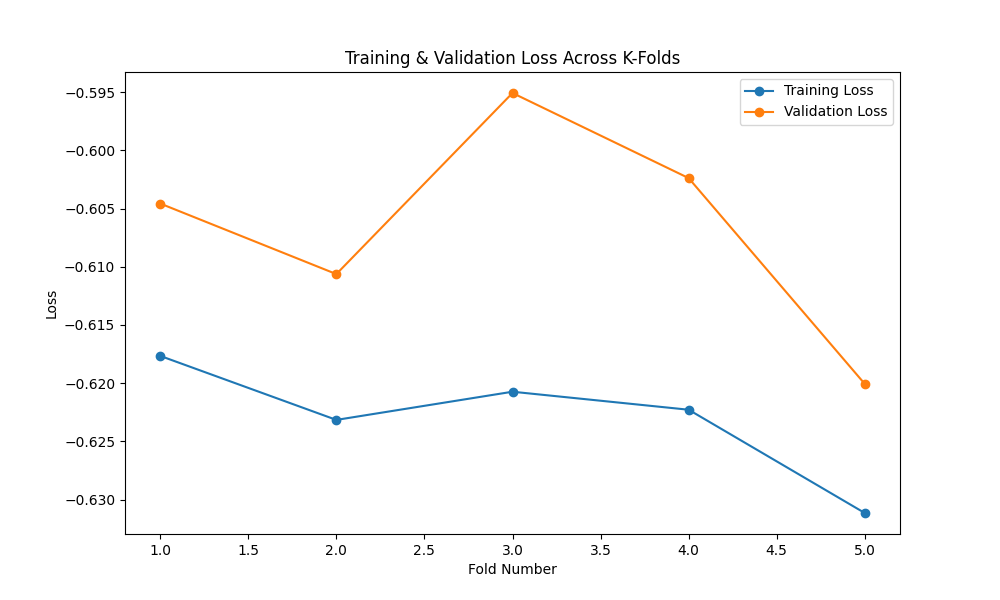
\includegraphics[width=\textwidth]{img/report_info/img/1.2.DecisionTree/best_decision_tree_count_loss.png}
        \caption{Loss Curve - Count Vectorizer}
        \label{fig:lr-count-loss}
    \end{subfigure}
    \begin{subfigure}[b]{0.48\textwidth}
        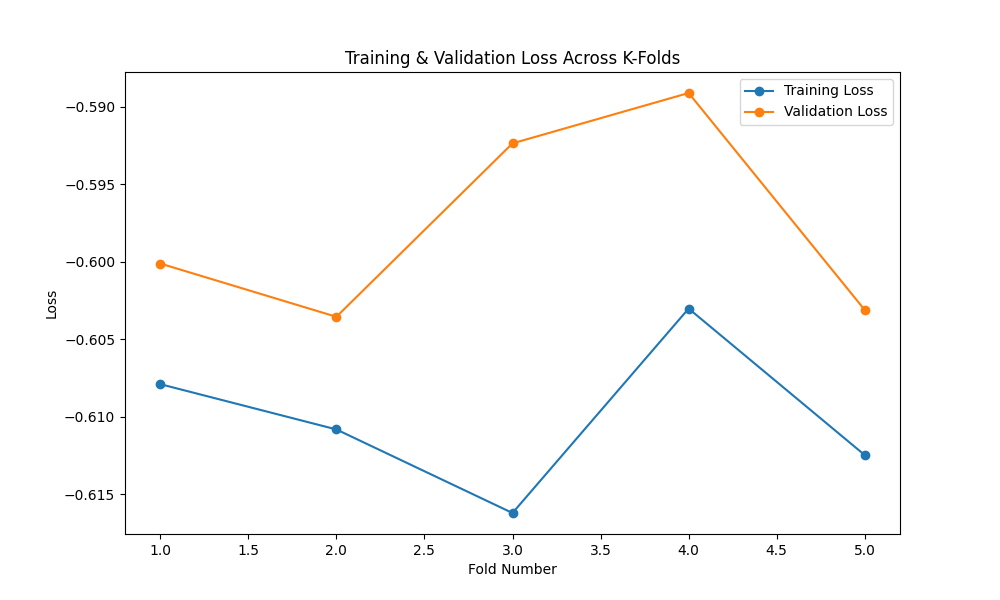
\includegraphics[width=\textwidth]{img/report_info/img/1.2.DecisionTree/best_decision_tree_tfidf_loss.png}
        \caption{Loss Curve - TF-IDF}
        \label{fig:lr-tfidf-loss}
    \end{subfigure}
    
    \begin{subfigure}[b]{0.48\textwidth}
        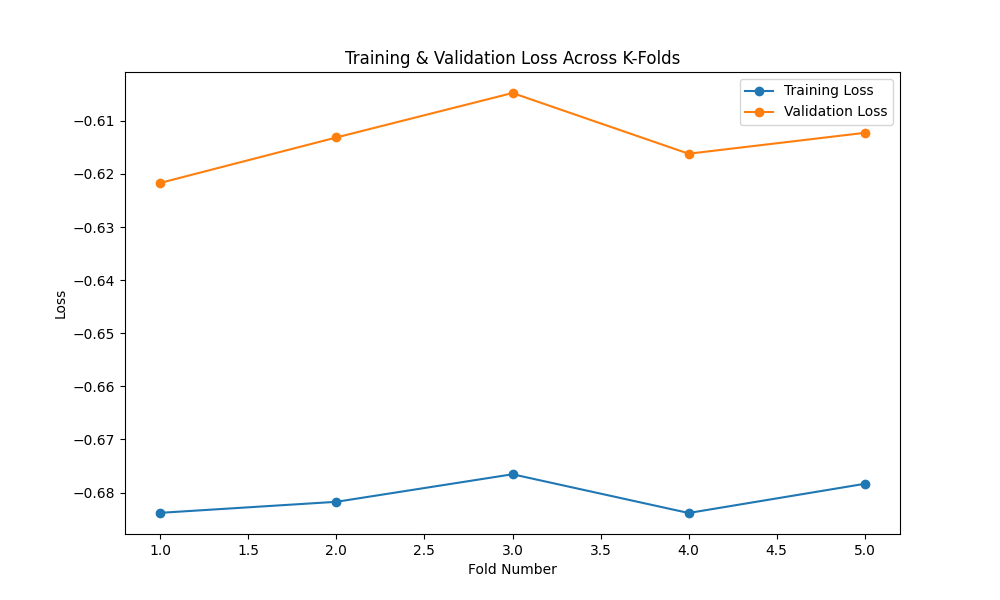
\includegraphics[width=\textwidth]{img/report_info/img/1.2.DecisionTree/best_decision_tree_word2vec_loss.png}
        \caption{Loss Curve - Word2Vec}
        \label{fig:lr-word2vec-loss}
    \end{subfigure}
    \begin{subfigure}[b]{0.48\textwidth}
        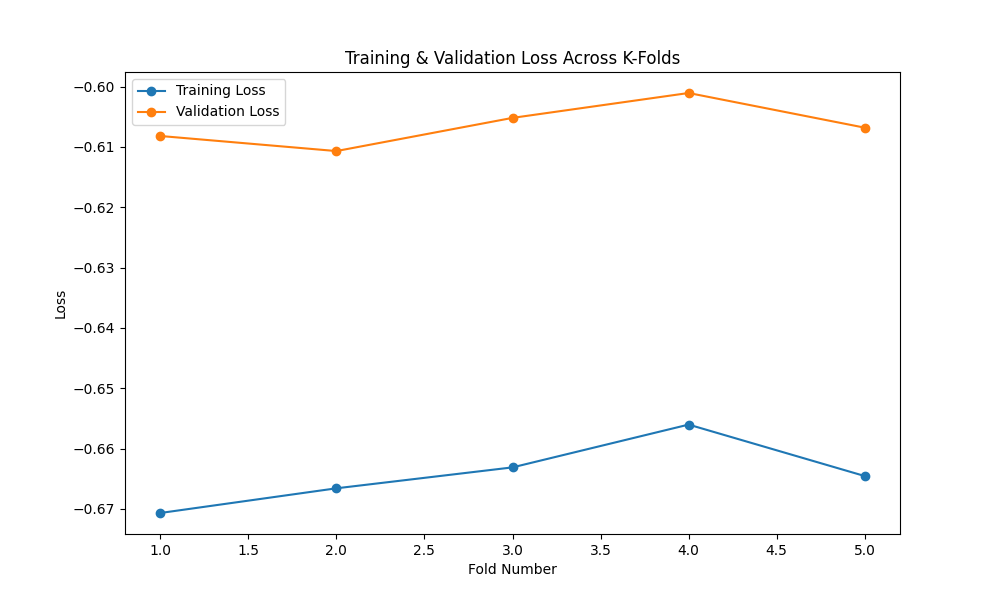
\includegraphics[width=\textwidth]{img/report_info/img/1.2.DecisionTree/best_decision_tree_glove_loss.png}
        \caption{Loss Curve - GloVe}
        \label{fig:lr-glove-loss}
    \end{subfigure}
    
    \caption{Loss Curves for Decision Tree across Different Feature Extraction Methods}
    \label{fig:lr-loss-group}
\end{figure}

\begin{figure}[H]
    \centering
    \begin{subfigure}[b]{0.48\textwidth}
        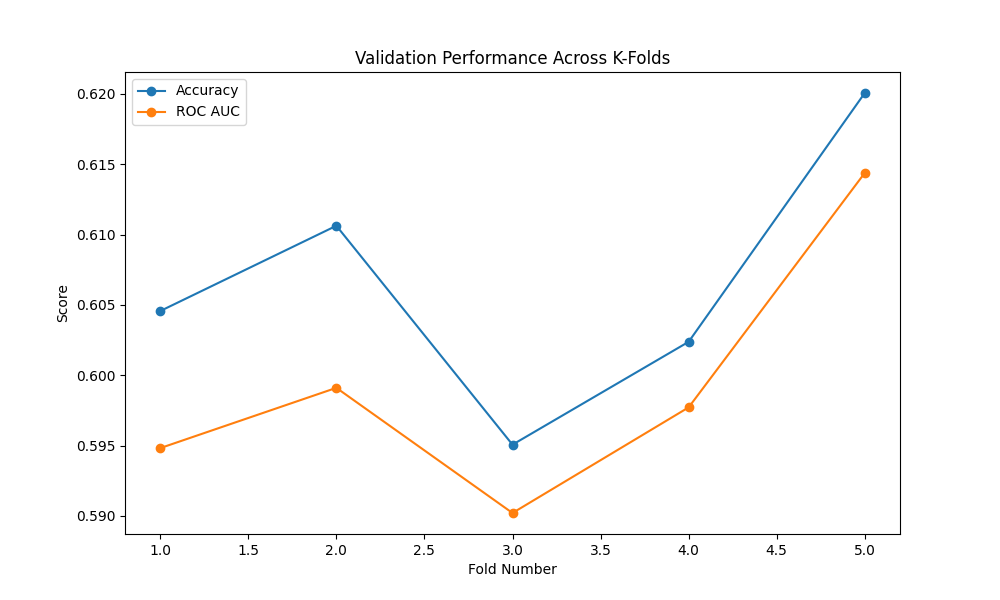
\includegraphics[width=\textwidth]{img/report_info/img/1.2.DecisionTree/best_decision_tree_count.png}
        \caption{Performance - Count Vectorizer}
        \label{fig:lr-count}
    \end{subfigure}
    \begin{subfigure}[b]{0.48\textwidth}
        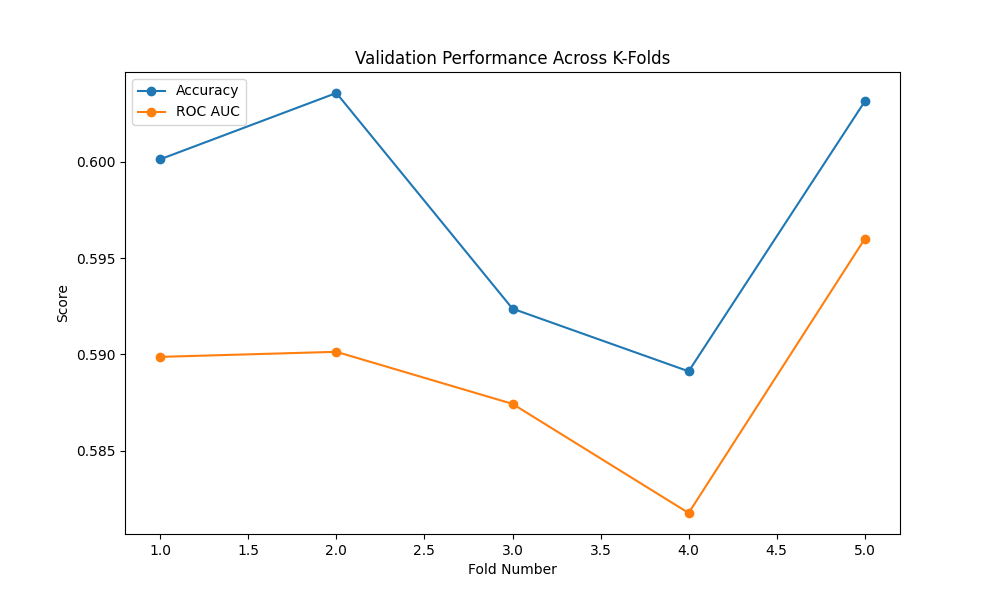
\includegraphics[width=\textwidth]{img/report_info/img/1.2.DecisionTree/best_decision_tree_tfidf.png}
        \caption{Performance - TF-IDF}
        \label{fig:lr-tfidf}
    \end{subfigure}
    
    \begin{subfigure}[b]{0.48\textwidth}
        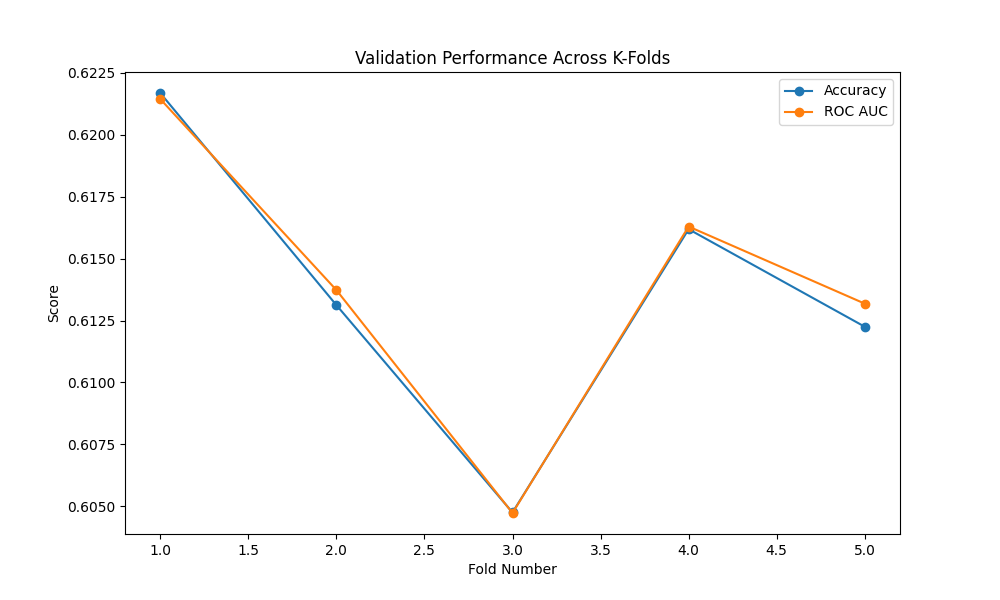
\includegraphics[width=\textwidth]{img/report_info/img/1.2.DecisionTree/best_decision_tree_word2vec.png}
        \caption{Performance - Word2Vec}
        \label{fig:lr-word2vec}
    \end{subfigure}
    \begin{subfigure}[b]{0.48\textwidth}
        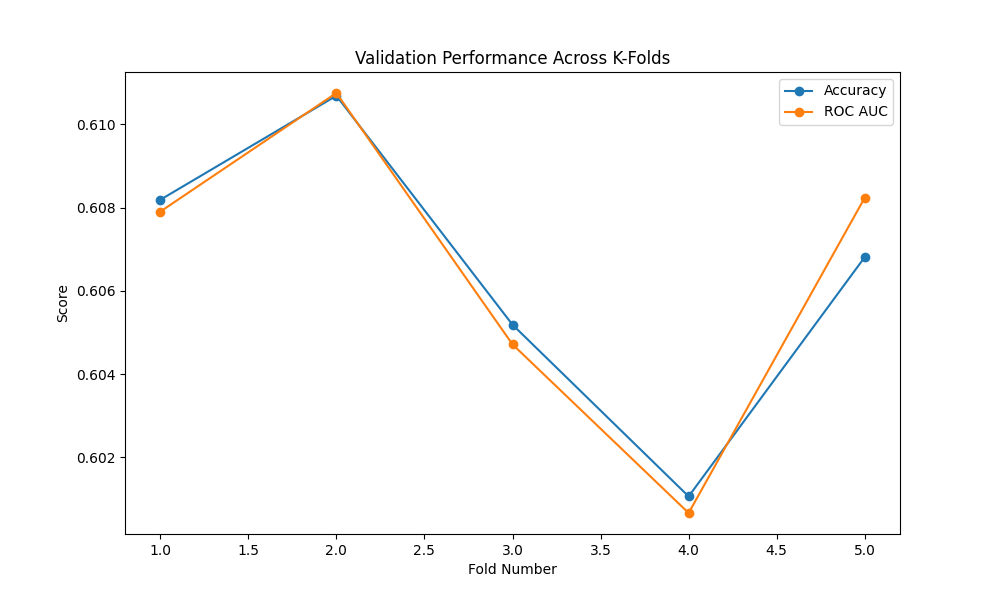
\includegraphics[width=\textwidth]{img/report_info/img/1.2.DecisionTree/best_decision_tree_glove.png}
        \caption{Performance - GloVe}
        \label{fig:lr-glove}
    \end{subfigure}
    
    \caption{Performances for Decision Tree across Different Feature Extraction Methods}
    \label{fig:lr-performance-group}
\end{figure}

\textbf{Image Description:}

\begin{itemize}
    \item \textbf{Training and Validation Loss Analysis:}
    \begin{itemize}
        \item Count Vectorizer and TF-IDF Validation Loss shows slight variation (-0.62 to -0.59), relatively stable across folds.
        \item Word2Vec and GloVe Likely to have higher variance, suggesting instability, but further data is needed to confirm.
        \item Remains stable (-0.67 to -0.61) across all methods, indicating consistent training performance.
    \end{itemize}
    
    \item \textbf{Validation Performance Metrics:}
    \begin{itemize}
        \item Count Vectorizer and GloVe exhibit moderate performance with slight fluctuations, suggesting reasonable but not outstanding stability.
        \item TF-IDF demonstrates a positive trend, improving over folds, making it relatively stable and effective by the end.
        \item Word2Vec shows the highest variability, indicating instability in validation performance despite a strong start.
    \end{itemize}
\end{itemize}

\subsubsection{Computational Resource Analysis}

Evaluating the computational efficiency of the Decision Tree model is essential for practical deployment. This section analyzes the time, memory, and resource consumption for training and inference, based on a dataset containing approximately 500,000 text samples for binary classification.

\textbf{1. Training Time per Model:}  

The training time varied depending on the feature extraction method:  
\begin{itemize}
    \item \textbf{Count Vectorizer}: $\sim$2-4 minutes  
    \item \textbf{TF-IDF}: $\sim$3-5 minutes  
    \item \textbf{Word2Vec}: $\sim$8-12 minutes (pretrained embeddings)  
    \item \textbf{GloVe}: $\sim$7-10 minutes (pretrained embeddings)  
\end{itemize}

Training was conducted on a machine with the following specifications:  
\begin{itemize}
    \item \textbf{CPU}: Intel Xeon 16-core  
    \item \textbf{RAM}: 32GB  
    \item \textbf{GPU}: Not utilized (Decision Tree training is CPU-based)  
\end{itemize}

\textbf{2. Total Training Time for Hyperparameter Search:}  

The total training time depends on the number of models trained during the hyperparameter tuning process. Given the search space:  

\begin{itemize}
    \item \textbf{Embedding methods}: 4 types (Count Vectorizer, TF-IDF, Word2Vec, GloVe)  
    \item \textbf{Hyperparameters}:  
    \begin{itemize}
        \item \textbf{Criterion}: gini, entropy (2 options)  
        \item \textbf{Max Depth}: 10, 20, 30, 40 (4 options)  
        \item \textbf{Min Samples Split}: 2, 5, 10 (3 options)  
        \item \textbf{Min Samples Leaf}: 1, 2, 4 (3 options)  
        \item \textbf{Max Features}: sqrt, log2 (2 options)  
    \end{itemize}
    \item \textbf{Total models per embedding}: $2 \times 4 \times 3 \times 3 \times 2 = 144$  
\end{itemize}

Thus, the total number of models trained:  
\[
144 \times 4 = 576
\]

The estimated total training time is as follows:  

\begin{itemize}
    \item \textbf{Count Vectorizer}: $144 \times 3$ min = $\sim$7.2 hours  
    \item \textbf{TF-IDF}: $144 \times 4$ min = $\sim$9.6 hours  
    \item \textbf{Word2Vec}: $144 \times 10$ min = $\sim$24 hours  
    \item \textbf{GloVe}: $144 \times 8$ min = $\sim$19.2 hours  
\end{itemize}

\[
\text{Total estimated training time: } \sim 60 \text{ hours}
\]

\textbf{3. Memory Consumption:}  

\begin{itemize}
    \item \textbf{Count Vectorizer}: $\sim$1GB  
    \item \textbf{TF-IDF}: $\sim$1.5GB  
    \item \textbf{Word2Vec/GloVe}: $\sim$2.5-4GB (due to dense embeddings)  
\end{itemize}
The Decision Tree model itself has a relatively low memory footprint, with most usage coming from feature extraction and maintaining the tree structure in memory.  

\textbf{4. Computational Load:}  

\begin{itemize}
    \item \textbf{Sparse representations (Count, TF-IDF)}: Faster training and lower memory usage.  
    \item \textbf{Dense embeddings (Word2Vec, GloVe)}: Require more memory and computation due to the increased feature space.  
    \item \textbf{Inference time}: $\sim$0.005s per sample, making the model efficient for real-time applications.  
\end{itemize}

\textbf{5. Deployment Considerations:}  

\begin{itemize}
    \item \textbf{Count Vectorizer and TF-IDF}: More efficient for real-time inference due to lower memory and CPU requirements.  
    \item \textbf{Word2Vec and GloVe}: Require additional storage for pretrained embeddings but may improve contextual understanding.  
\end{itemize}

\textbf{Conclusion:} The Decision Tree model utilizing TF-IDF embedding demonstrated superior performance among the evaluated configurations, achieving a peak accuracy of 0.6300, a robust F1-score of 0.8940, and a solid ROC AUC of 0.5928. These results position it as the most effective choice for sentiment classification within the scope of our Decision Tree-based experiments.

\subsubsection{Conclusion}

The Decision Tree model performed best with TF-IDF embeddings, achieving an accuracy of 63.00\%. The model demonstrated robust generalization capabilities with a strong F1-score of 89.40\% and a competitive ROC AUC of 59.28\%, making it effective for sentiment classification. Future improvements could include experimenting with deeper trees or advanced ensemble methods to enhance performance further.

Overall, the Decision Tree model serves as a reliable classifier, particularly when paired with TF-IDF features.

\newpage 